% 
% ---------------------------------------------------------------
% Copyright (C) 2012-2018 Gang Li
% ---------------------------------------------------------------
%
% This work is the default powerdot-tuliplab style test file and may be
% distributed and/or modified under the conditions of the LaTeX Project Public
% License, either version 1.3 of this license or (at your option) any later
% version. The latest version of this license is in
% http://www.latex-project.org/lppl.txt and version 1.3 or later is part of all
% distributions of LaTeX version 2003/12/01 or later.
%
% This work has the LPPL maintenance status "maintained".
%
% This Current Maintainer of this work is Gang Li.
%
%

\documentclass[
 size=12pt,
 paper=smartboard, %a4paper, smartboard, screen
 mode=present, %present, handout, print
 display=slides, % slidesnotes, notes, slides
% nohandoutpagebreaks,
% pauseslide,
style=tuliplab,
% nopagebreaks,clock
% hlentries=true,
% hlsections = true,
pauseslide,
fleqn,leqno]{powerdot}

\hypersetup{pdfpagemode=FullScreen}
% \usepackage[toc,highlight,blackslide,slidesonly,sounds,HA]{HA-prosper}

\usepackage{amssymb}
\usepackage{amsmath} 
\usepackage{rotating}
\usepackage{graphicx}
\usepackage{boxedminipage}
\usepackage{media9}
\usepackage{rotate}
\usepackage{calc}
\usepackage[absolute]{textpos}
\usepackage{psfrag,overpic}
\usepackage{fouriernc}
\usepackage{pstricks,pst-node,pst-text,pst-3d,pst-grad}
\usepackage{moreverb,epsfig,color,subfigure}
\usepackage{color}
\usepackage{pstricks}
\usepackage{pstricks-add}
\usepackage{pst-text}
\usepackage{pst-node, pst-tree}
\usepackage{booktabs}
\usepackage{etex}
\usepackage{breqn}
\usepackage{multirow}
\usepackage{gitinfo2}

\usepackage{listings}
\lstset{frameround=fttt, 
frame=trBL, 
stringstyle=\ttfamily,
backgroundcolor=\color{yellow!20},
basicstyle=\footnotesize\ttfamily}
\lstnewenvironment{code}{
\lstset{frame=single,escapeinside=`',
backgroundcolor=\color{yellow!20},
basicstyle=\footnotesize\ttfamily}
}{}


\usepackage{fouriernc}
\usepackage{hyperref}

%%%%%%%%%%%%%%%%%%%%%%%%%%%%%%%%%%%%%%%%%%%%%%%%%%%%%%%%%%%%%%%%%%%%%%%%
% title
% TODO: Customize to your Own Title, Name, Address
%
\title{FLIP01 MIDTERM PRESENTATION}
\author{
Zebin Ju
\\
Xi'an Shiyou University 
% \href{mailto:gangli@acm.org}{gangli@acm.org}
% \and % more authors
}
\date{\today}


% Customize the setting of slides
\pdsetup{
% theslide=\arabic{slide}~/~\pageref*{lastslide},
% theslide=\arabic{slide},
rf=\href{http://www.tulip.org.au}{
Last Changed by: \textsc{\gitCommitterName}\ \gitVtagn-\gitAbbrevHash\ (\gitAuthorDate)
},
cf={FLIP01 MIDTERM PRESENTATION},
%trans=Fade,
%list={labelsep=1em,leftmargin=*,itemsep=0pt,topsep=5pt,parsep=0pt},
% counters={theorem,lemma},
% randomdots,dmaxdots=80
}


\begin{document}

\maketitle 
\begin{slide}[toc=,bm=]{Overview}
  \tableofcontents[content=sections]
\end{slide}

  \section{Problem Description}

  \begin{slide}{Description}
  %\tableofcontents[content=currentsection,type=1]
 \hspace{0.5cm}  Rotten tomato movie review data set is a movie review corpus for emotional analysis. 
 It is an opportunity for us to build your idea of Emotional Analysis on rotten tomato data set. It is required to mark phrases with five levels of values: negative, some negative, neutral, some positive, positive. Negative sentences, satire, conciseness, language ambiguity and other obstacles make this task very challenging.
  \end{slide}
  %\begin{slide}{The overview of the question }
    %\vspace{2cm}
    %\setlength{\parindent}{1.5em}
    %You are given 5 years of store-item sales data, and asked to predict 3 months of sales for 50 different items at 10 different stores.
  %\end{slide}
  %\begin{slide}{Data Set}
    %\begin{itemize}
      %\begin{itemize}
    %\item train data
    %\begin{table}[htbp]  \centering
      %\caption{The head of the train data}
      %\label{tbl:data information}
      %\begin{tabular}{ccccccc}
       % \hline
        % after \\: \hline or \cline{col1-col2} \cline{col3-col4} ...
       % & cuisine & id & igredients\\
       % \hline
       % 0 & greek       & 10259 & [romaine lettuce, black olives, grape tomatoes... \\
       % 1 & southern_us & 25693 & [plain flour, ground pepper, salt, tomatoes, g... \\
       % 2 & filipino    & 20130 & [eggs, pepper, salt, mayonaise, cooking oil, g... \\
       % 3 & indian      & 22213 & [water, vegetable oil, wheat, salt] \\
       % 4 & indian      & 13162 & [black pepper, shallots, cornflour, cayenne pe... \\
       % \hline 
        %\bottomrule
      %\end{tabular}
    %\end{table}
    \

  %\item Display the data set 
 % \begin{table}[htbp]  \centering
    %\caption{The head of the test data}
    %\label{tbl:data information}
    %\begin{tabular}{ccccccc}
      % after \\: \hline or \cline{col1-col2} \cline{col3-col4} ...
     % & id & igredients\\
      %\hline
      %0  & 18009 & [baking powder, eggs, all-purpose flour, raisi... \\
      %1  & 28583 & [sugar, egg yolks, corn starch, cream of tarta... \\
      %2  & 41580 & [sausage links, fennel bulb, fronds, olive oil... \\
     % 3  & 29752 & [meat cuts, file powder, smoked sausage, okra,... \\
      %4  & 35687 & [ground black pepper, salt, sausage casings, l... \\
      %\hline 
      %\bottomrule
   % \end{tabular}
  %\end{table}
  %\end{itemize}
%\end{slide}
 % \begin{slide}[toc=,bm=]{Overview}
    %\tableofcontents[content=sections]
    %\end{slide}
    %\section{Second section}
    %\begin{slide}[toc=,bm=]{Main contents}
    %\tableofcontents[content=currentsection,type=1]
    %\end{slide}
    %\begin{slide}{Problem analysis by using data visualization}
      %\begin{itemize}
      %\item List the directories and files and load  data set
      %\item The introduction of the data set
      %\item Plot statistical charts and see the sale pattern
      %\item Variation in scale of the sale transacted
      %\item Store total sales
      %\item Item total sales
      %\item All store's performance
      %\item Individual pattern of store's and item's sales
      %\end{itemize}
    %\end{slide} 


    \section{Problem Analysis}
  
\begin{slide}{Data Analysis}
  \hspace{0.5cm}  The dataset consists of tab delimited files and phrases in the rotten tomatoes dataset. Each phrase has a phraseid. Each sentence has a sentenceid.\\
  
  \vspace{1cm}
\begin{itemize}
  \item 0 for negative
  \item 1 for somewhat negative
  \item 2 for neutral
  \item 3 for somewhat positive
  \item 4 for positive
\end{itemize}

%The output example:\\
%\vspace{1cm}
%\hspace{5cm}array([[0,0,0,...0,0,0],\\\hspace{6.25cm}[0,0,0,...0,0,0],\\\hspace{6.25cm}[0,0,0,...0,0,0],\\\hspace{6.25cm}...\\\hspace{6.25cm}[0,0,0,...0,0,0],\\\hspace{6.25cm}[0,0,0,...0,0,0],\\\hspace{6.25cm}[0,0,0,...0,0,0]],\\\hspace{6.05cm})
%\end{slide}
%\begin{slide}[toc=,bm=]{Data Glance}
  %\begin{figure}[ht]%插入图片
    %\centering%用于居中
    %\includegraphics[scale=0.9]{D:/software/flip01/pictures/train.eps}
    %\caption{Data characteristics table}%图片标题
    %\end{figure}
\end{slide}  
\begin{slide}{Data Glance}
  \hspace{0.5cm}  The following table shows the data characteristics.\\
  
  \vspace{1cm}
  \begin{figure}[ht]%插入图片
    \centering%用于居中
    \includegraphics[scale=1]{D:/software/flip01/pictures/train.eps}
    \caption{data characteristics table}%图片标题
    \end{figure}
\end{slide}

%\begin{slide}{Type Of Review}
  %\begin{table}[htbp]  \centering
      %\caption{The head of the train data}
      %\label{tbl:data information}
      %\begin{tabular}{ccccccc}
       % \hline
        % after \\: \hline or \cline{col1-col2} \cline{col3-col4} ...
       % & cuisine & id & igredients\\
       % \hline
       % 0 & greek       & 10259 & [romaine lettuce, black olives, grape tomatoes... \\
       % 1 & southern_us & 25693 & [plain flour, ground pepper, salt, tomatoes, g... \\
       % 2 & filipino    & 20130 & [eggs, pepper, salt, mayonaise, cooking oil, g... \\
       % 3 & indian      & 22213 & [water, vegetable oil, wheat, salt] \\
       % 4 & indian      & 13162 & [black pepper, shallots, cornflour, cayenne pe... \\
       % \hline 
        %\bottomrule
      %\end{tabular}
    %\end{table}
    \
  %\hspace{0.5cm}  Next, we can see the category distribution of comments. From the figure, we can see that emotion tag 2, that is, the most neutral comments.\\
  
  %\vspace{1cm}
  
%\end{slide}

\begin{slide}{Type Of Review}
  \hspace{0.5cm}  Next, we can see the category distribution of comments. From the figure, we can see that emotion tag 2, that is, the most neutral comments. \\
  
  \vspace{1cm}
  \begin{figure}[ht]%插入图片
   \centering%用于居中
   \includegraphics[scale=0.99]{D:/software/flip01/pictures/review.eps}
   \caption{type of review}%图片标题
   \end{figure}
\end{slide}
%\begin{slide}{Plot statistical charts and see the sale pattern} 
%By using the matplotlib to plot the photoes which describe the sale pattern
%\vspace{1cm}
%\begin{figure}[ht]%插入图片
  %\centering%用于居中
  %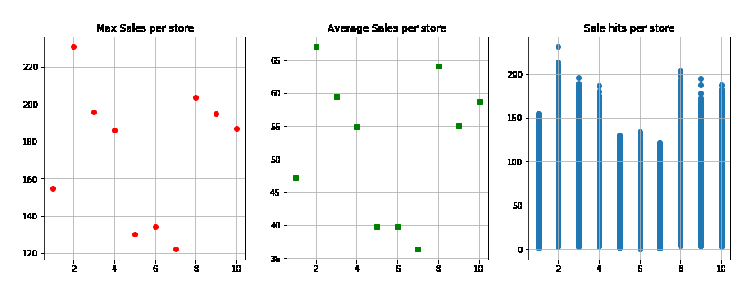
\includegraphics[scale=0.9]{E:/tulip-flip/templatex-master/powerdot-tuliplab/logos/0003.eps}
  %\caption{Displaying the sale pattern}%图片标题
  %\end{figure}
  %\vspace{0.5cm}
%From the figures we can know that 2nd store is the topper and 7th store is the least revenue generating one
%\end{slide}

%\begin{slide}{Variation in scale of the sale transacted}
%Displaying the distribution of sales volume 
%\vspace{1cm}
%\begin{figure}[ht]%插入图片
  %\centering%用于居中
  %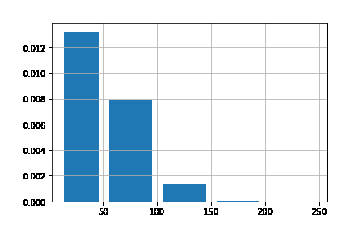
\includegraphics[scale=1.0]{E:/tulip-flip/templatex-master/powerdot-tuliplab/logos/0004.eps}
  %\caption{sales volume's distribution}%图片标题
  %\end{figure}
  %\vspace{1cm}
  %From this figure we can know that more and more sales volume is belong to [0,50]
%\end{slide}

%\begin{slide}{Store total sales}
%Displaying the total sales of the stores 
%\vspace{1.0cm}
%\begin{figure}[ht]%插入图片
  %\centering%用于居中
  %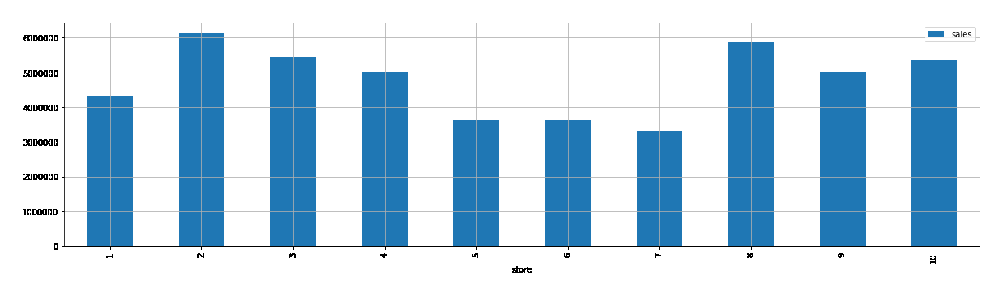
\includegraphics[scale=1.0]{E:/tulip-flip/templatex-master/powerdot-tuliplab/logos/0005.eps}
  %\caption{The total sales of all stores}%图片标题
  %\end{figure}
  %\vspace{0.5cm}
  %From this figure we can know that 2nd store is the topper of the all stores
%\end{slide}

%\begin{slide}{Item total sales}
  %Displaying the total sales of the items 
  %\vspace{0.8cm}
  %\begin{figure}[ht]%插入图片
    %\centering%用于居中
    %\includegraphics[scale=0.7]{E:/tulip-flip/templatex-master/powerdot-tuliplab/logos/0006.eps}
    %\caption{The total sales of all items}%图片标题
   % \end{figure}
    %\vspace{0.3cm}
   % From this figure we can know the total sales of all items.Obviously,we can know every item's sales
%\end{slide}

%\begin{slide}{All store's performance}
%Displaying the all store's performance over the time
%\vspace{1cm}
%\begin{figure}[ht]%插入图片
  %\centering%用于居中
  %\includegraphics[scale=0.7]{E:/tulip-flip/templatex-master/powerdot-tuliplab/logos/0007.eps}
  %\caption{The performance of all stores}%图片标题
  %\end{figure}
  %From this figure we can know every stores sales changing overtime
%\end{slide}

%\begin{slide}{All item's performance}
  %Displaying the all items' performance over the time
  %\vspace{1.2cm}
  %\begin{figure}[ht]%插入图片
    %\centering%用于居中
    %\includegraphics[scale=0.7]{E:/tulip-flip/templatex-master/powerdot-tuliplab/logos/0008.eps}
    %\caption{The performance of all stores items}%图片标题
    %\end{figure}
    %From this figure we can know every item sales changing overtime 
  %\end{slide}

%\begin{slide}{Individual pattern of store's and item's sale}
%Displaying the performance of the individual score and item
%\vspace{1cm}
%\begin{figure}[ht]%插入图片
  %\centering%用于居中
  %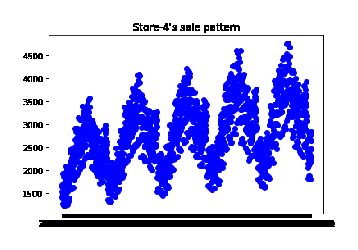
\includegraphics[scale=0.9]{E:/tulip-flip/templatex-master/powerdot-tuliplab/logos/0009.eps}
  %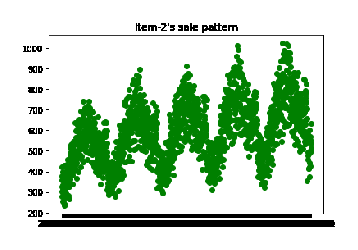
\includegraphics[scale=0.9]{E:/tulip-flip/templatex-master/powerdot-tuliplab/logos/0010.eps}
  %\caption{The performance of the individual store and item}%图片标题
  %\end{figure}
  %\vspace{0.8cm}
  %From this figure we can know individual pattern of item's sale and store's sale
%\end{slide}
\section{Text Feature Extraction}

\begin{slide}[toc=,bm=]{Text Feature Extraction}
  \hspace{0.5cm}  It is the process of transforming text data into feature vector. Machine learning algorithm often can't directly process text data, so it needs to transform text data into numerical data.
\begin{itemize}
  \item CountVectorizer \ 

 % There are many machine learning methods for solving regression problems. This moment I will choose the lightGBM model
  \item  TfidfVectorizer
  %\[SMAPE=\frac{100\%}{n}\sum_{t=1}^n\frac{|F_t-A_t|}{(|A_t|+|F_t|)/2} \]
\end{itemize}
\end{slide}

%\begin{slide}[toc=,bm=]{Forcasting}
%\begin{itemize}
 % \item Divide training data and test data
  %\item Do a model training
 % \item Model prediction
 % \item Model evaluation
  %\item Re-train model
  %\item Feature importance
 %\item test predations
%\end{itemize}
%\end{slide}

%\begin{slide}[toc=,bm=]{Forcasting}
  %\begin{figure}[ht]%插入图片
    %\centering%用于居左
    %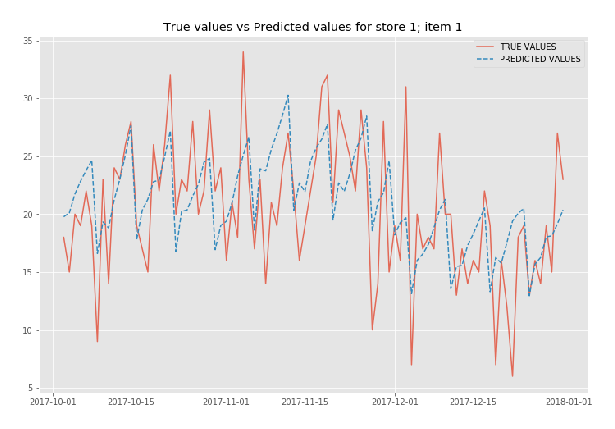
\includegraphics[scale=0.7]{E:/tulip-flip/templatex-master/powerdot-tuliplab/logos/012.eps}
   % \caption{The value vs predict}%图片标题
    %\end{figure}
%\vspace{1cm}
%Figure 8 is the first prediction based on the model.
%\end{slide}

%\begin{slide}[toc=,bm=]{Forcasting}
  %\begin{figure}[ht]%插入图片
    %\centering%用于居左
    %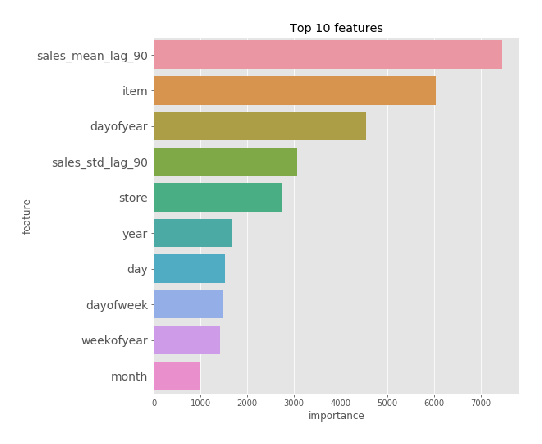
\includegraphics[scale=0.7]{E:/tulip-flip/templatex-master/powerdot-tuliplab/logos/013.eps}
    %\caption{Top 10 importabce features}%图片标题
    %\end{figure}
%\vspace{1cm}
%Figure 9 shows ten features with high feature importance.
%\end{slide}


%\begin{slide}[toc=,bm=]{Forcasting}
  %\begin{figure}[ht]%插入图片
    %\centering%用于居中
   %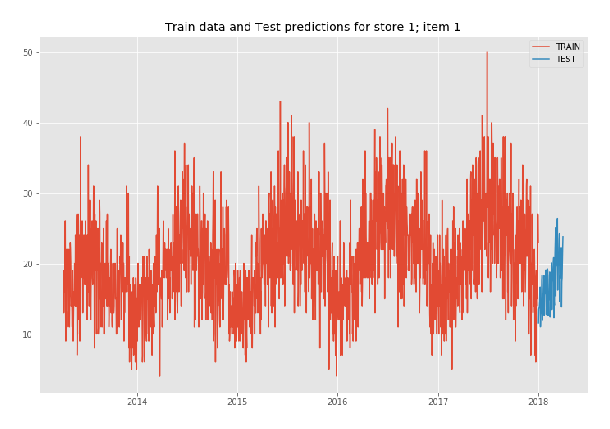
\includegraphics[scale=0.7]{E:/tulip-flip/templatex-master/powerdot-tuliplab/logos/014.eps}
   % \caption{The test prediction}%图片标题
   %\end{figure}
%\vspace{1cm}
%Figure 10 is a new prediction based on the model to get the results needed for this problem.
%\end{slide}

\section{Methods}
\begin{slide}[toc=,bm=]{Naive Bayes}
  \hspace{0.5cm}  Naive Bayes is a classification algorithm based on probability theory, which can predict classification by considering feature probability. 
  \begin{itemize}
    \item CountVectorizer:0.6715045495322312 \ 

    \item TfidfVectorizer:0.6308070613866461
    \end{itemize}
    %\[SMAPE=\frac{100\%}{n}\sum_{t=1}^n\frac{|F_t-A_t|}{(|A_t|+|F_t|)/2} \]
   % \begin{figure}[ht]%插入图片
      %\centering%用于居中
      %\includegraphics[scale=1]{D:/software/flip01/pictures/cv Naive Bayes.eps}
      %\includegraphics[scale=1]{D:/software/flip01/pictures/tv Naive Bayes.eps}
     % \caption{naive bayes}%图片标题
     % \end{figure}
 
     
     \begin{figure}[ht]%插入图片
      \centering%用于居中
      \includegraphics[scale=1.0]{D:/software/flip01/pictures/cvBayes.eps}
      \includegraphics[scale=1.0]{D:/software/flip01/pictures/tvBayes.eps}
      \caption{naive bayes}%图片标题
      \end{figure} 
    \end{slide}
  %\begin{description}
 % \item[Data Analysis] Using visual methods to find connections and features within the dataset.
  %\item[Feature Engineering] Find and extract important features. 
  %\item[Modeling] Choose the suitable model parameters.
  %\item[Prospcting] I woule like to select multiple models for comparison later.
%\end{description}
\begin{slide}[toc=,bm=]{Logistic Regression}
  \hspace{0.5cm}  Logical regression can solve the problem of two categories, but it can also solve the problem of multiple categories.
  \begin{itemize}
    \item CountVectorizer:0.7002354863514033 \ 

    \item TfidfVectorizer:0.6662581699346405
    \end{itemize}
    %\[SMAPE=\frac{100\%}{n}\sum_{t=1}^n\frac{|F_t-A_t|}{(|A_t|+|F_t|)/2} \]
    \begin{figure}[ht]%插入图片
      \centering%用于居中
      \includegraphics[scale=1]{D:/software/flip01/pictures/cvLogistic.eps}
      \includegraphics[scale=1]{D:/software/flip01/pictures/tvLogistic.eps}
      \caption{logistic regression}%图片标题
      \end{figure}
 
    \end{slide}

\section{The Ending}


%\begin{slide}[toc=,bm=]{}
  %\tableofcontents[content=sections]
  %\end{slide}
  %\section{Third section}
  %\begin{slide}[toc=,bm=]{Acknowledge}
  %\tableofcontents[content=currentsection,type=1]
  %\end{slide}
%\begin{slide}{Acknowledge}
%\vspace{3.5cm}
%\centering
%\huge
%\textit{Thank you for watching the slides} 
%\end{slide}
\end{document}

\endinput
